\chapter{Réalisation et implémentation}
\label{chap:realisation}

\section{Introduction}

Ce chapitre présente la réalisation concrète de l'architecture sécurisée définie au chapitre précédent. Il décrit successivement la vue d'ensemble du système, la topologie réseau déployée sous GNS3 (segmentation VLAN, routage, pare-feu), le déploiement de l'infrastructure à clés publiques HashiCorp Vault avec sa hiérarchie de certification à deux niveaux, et la sécurisation du broker MQTT Mosquitto en TLS~1.3 strict avec authentification mutuelle. Chaque sous-système est documenté avec ses paramètres clés, ses interfaces et ses livrables ; les configurations exhaustives sont reportées en annexes.

\section{Vue d'ensemble de l'architecture}

L'architecture retenue est basée sur une approche \textbf{défense en profondeur} (\textit{defense in depth}) : chaque couche de l'écosystème dispose de ses propres mécanismes de sécurité, de sorte qu'une compromission partielle ne compromet pas l'ensemble du système. La figure~\ref{fig:archi_generale} présente la vue d'ensemble, organisée en cinq zones de sécurité distinctes.

\begin{figure}[H]
  \centering
  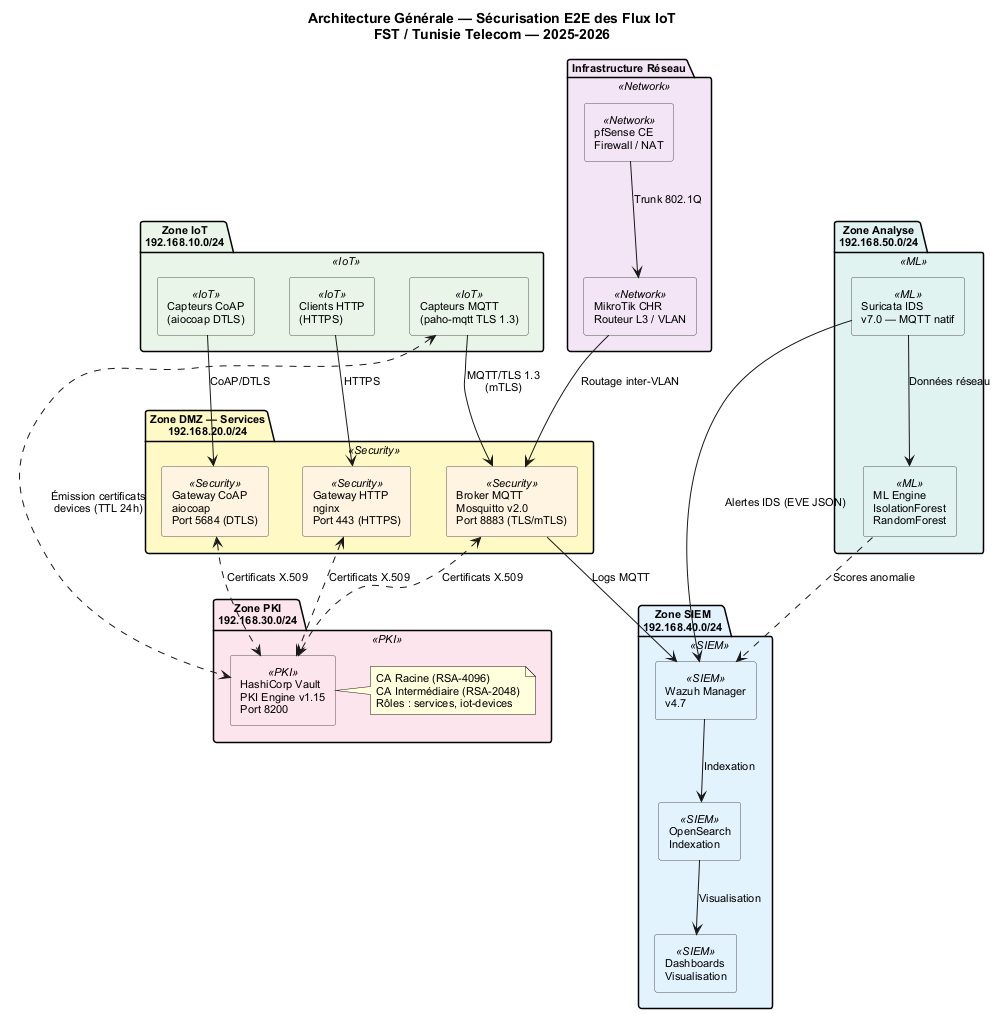
\includegraphics[width=\textwidth]{diagrams/diag-architecture-generale.png}
  \caption{Architecture générale de l'écosystème IoT sécurisé}
  \label{fig:archi_generale}
\end{figure}

Le diagramme de composants logiciels de la figure~\ref{fig:composants} détaille les interfaces de communication, avec les protocoles et ports utilisés entre chaque élément.

\begin{figure}[H]
  \centering
  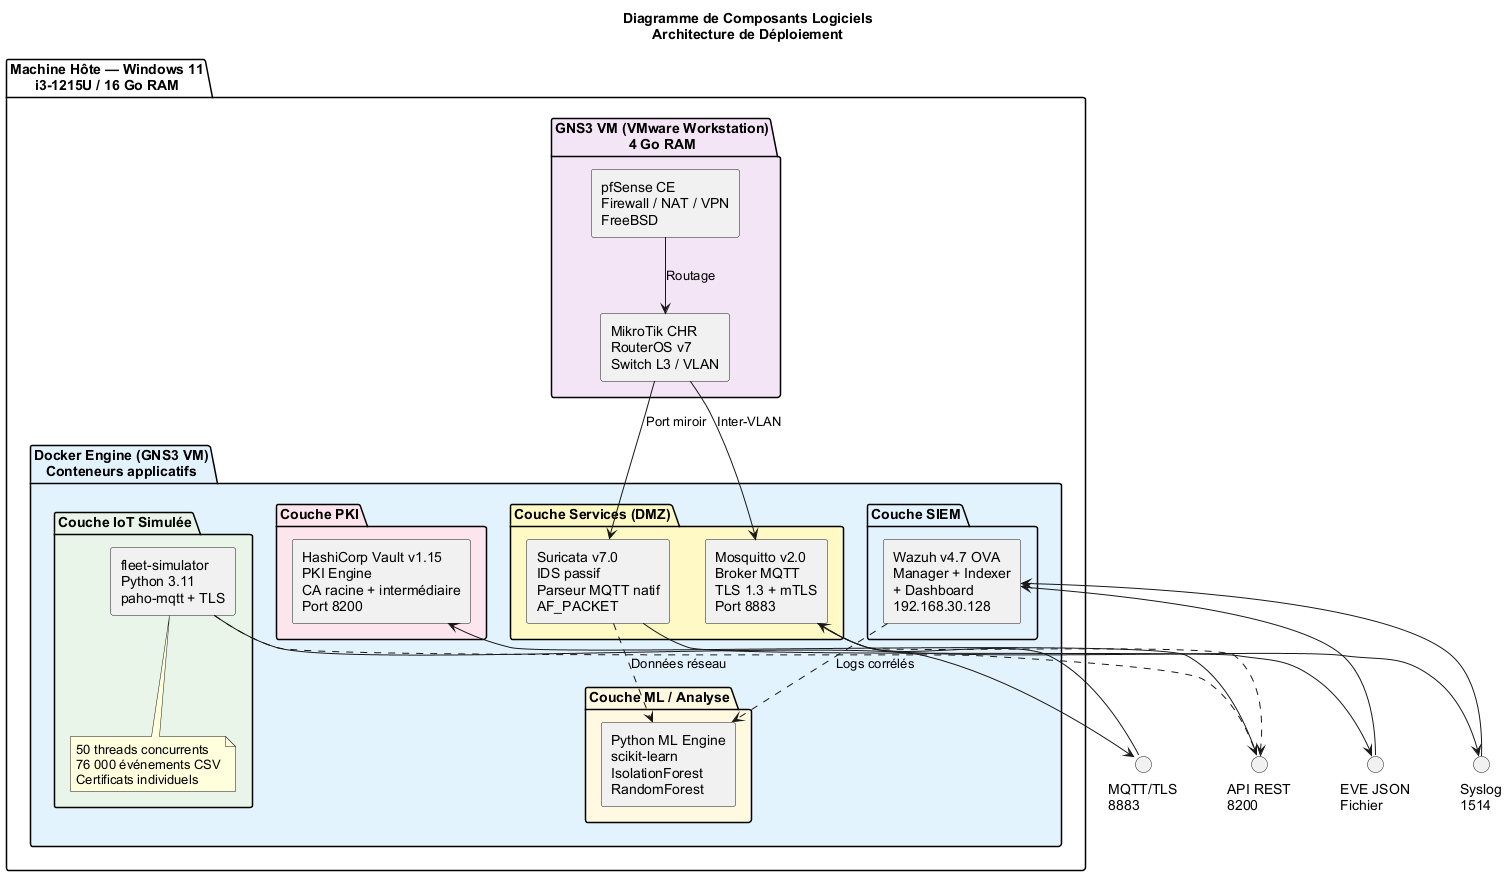
\includegraphics[width=\textwidth]{diagrams/diag-composants.png}
  \caption{Diagramme de composants logiciels et interfaces}
  \label{fig:composants}
\end{figure}

Le flux de données de bout en bout suit huit étapes : (1)~le dispositif demande un certificat à Vault, (2)~Vault émet un certificat X.509 valide 24~heures, (3)~le dispositif établit une connexion TLS~1.3 avec Mosquitto, (4)~Mosquitto valide la chaîne et applique l'ACL, (5)~les messages sont publiés sur les topics autorisés, (6)~Suricata inspecte le trafic et génère des alertes, (7)~Wazuh ingère et corrèle les alertes, (8)~le pipeline ML analyse les métriques pour détecter des anomalies. Le diagramme de séquence de la figure~\ref{fig:flux_e2e} illustre ce flux.

\begin{figure}[H]
  \centering
  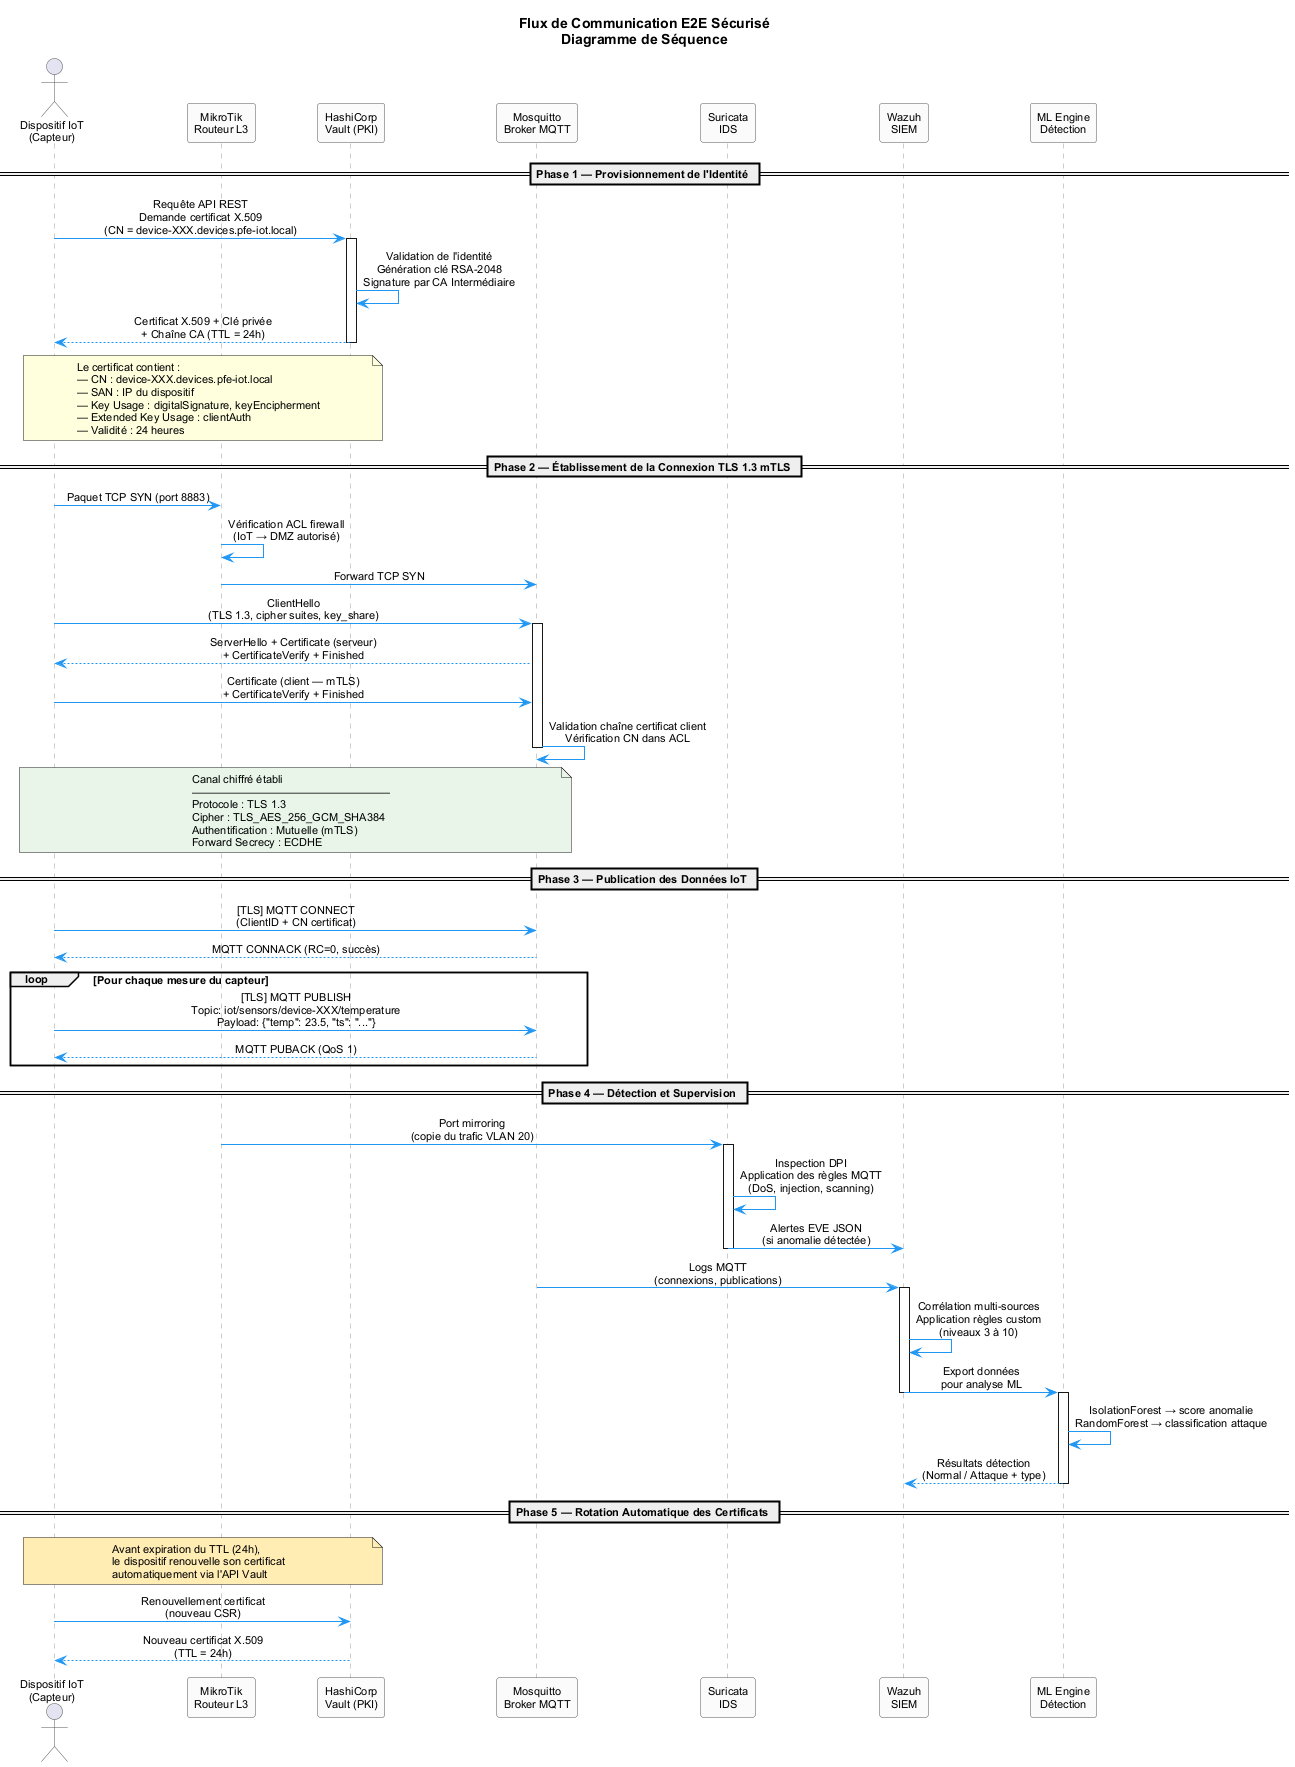
\includegraphics[width=\textwidth]{diagrams/diag-flux-e2e.png}
  \caption{Flux E2E sécurisé -- diagramme de séquence}
  \label{fig:flux_e2e}
\end{figure}

\section{Topologie réseau GNS3}

La simulation réseau est réalisée sous \textbf{GNS3} (Graphical Network Simulator 3) avec VMware Workstation Pro comme hyperviseur~\cite{gns3_docs}. La topologie est segmentée en trois VLANs isolés par un routeur MikroTik CHR, conformément au plan d'adressage du tableau~\ref{tab:adressage}.

\begin{table}[H]
\centering
\caption{Plan d'adressage de la topologie GNS3}
\label{tab:adressage}
\begin{tabular}{lllp{5cm}}
\toprule
\textbf{Réseau} & \textbf{CIDR} & \textbf{Composants} & \textbf{Rôle} \\
\midrule
IoT Devices & 192.168.10.0/24 & fleet-simulator, capteurs & Zone dispositifs -- trafic MQTT \\
Services & 192.168.20.0/24 & Mosquitto, Vault, Suricata & Zone services sécurisés \\
Management & 192.168.30.0/24 & Wazuh OVA & Zone administration et SIEM \\
\bottomrule
\end{tabular}
\end{table}

\begin{figure}[H]
  \centering
  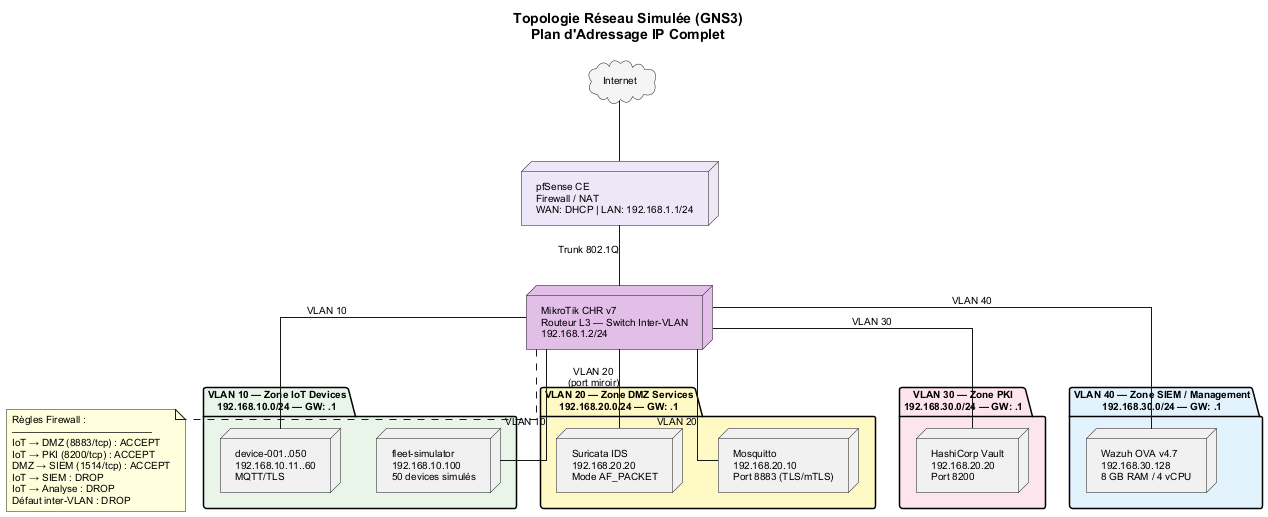
\includegraphics[width=\textwidth]{diagrams/diag-topologie-reseau.png}
  \caption{Topologie réseau détaillée}
  \label{fig:topologie_reseau}
\end{figure}

Un routeur \textbf{MikroTik CHR} (RouterOS~v7) assure le routage inter-VLAN et implémente les règles de pare-feu : autorisation explicite du port 8883 (MQTT/TLS) de la zone IoT vers la zone Services, blocage de tout trafic direct IoT~$\to$~Management, et NAT masquerade pour l'accès Internet. Un pare-feu \textbf{pfSense~CE} protège le périmètre externe de l'environnement simulé.

\begin{figure}[H]
  \centering
  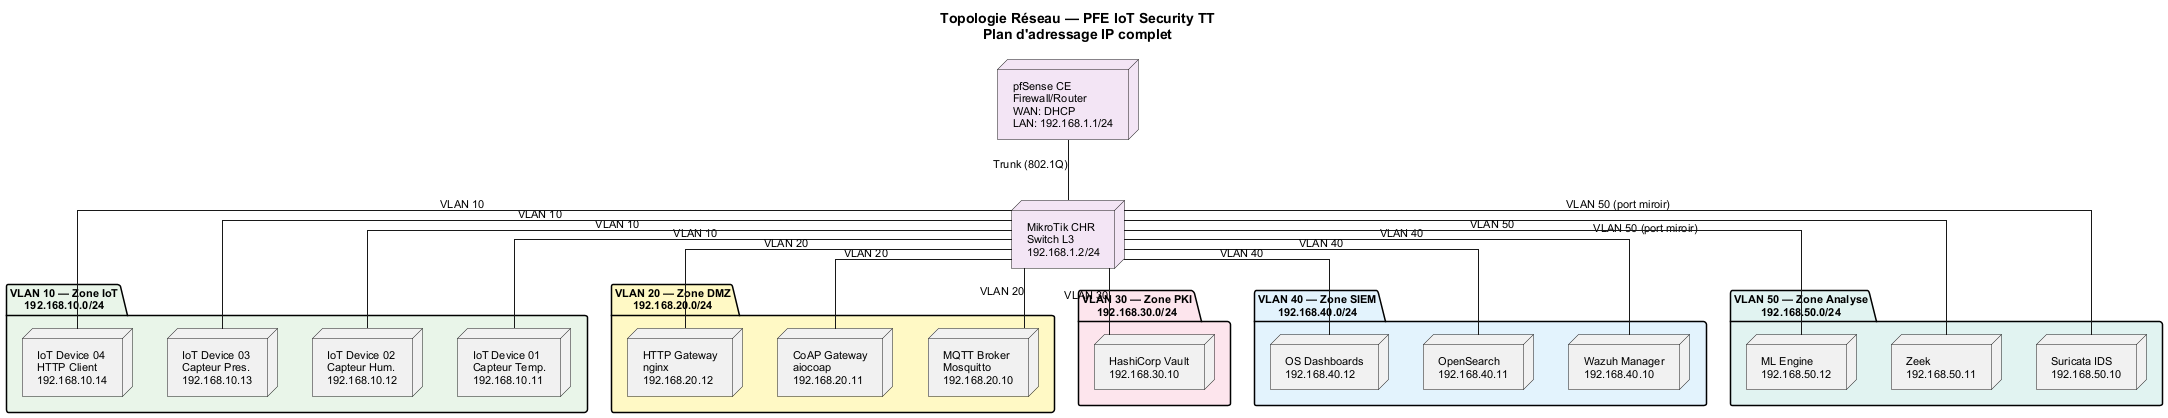
\includegraphics[width=\textwidth]{figures/gns3-topology.png}
  \caption{Topologie réseau dans l'interface GNS3}
  \label{fig:gns3_topology}
\end{figure}

Le diagramme de déploiement de la figure~\ref{fig:deploiement} présente l'ensemble des nœuds physiques et virtuels de l'infrastructure ainsi que les artefacts logiciels déployés sur chacun.

\begin{figure}[H]
  \centering
  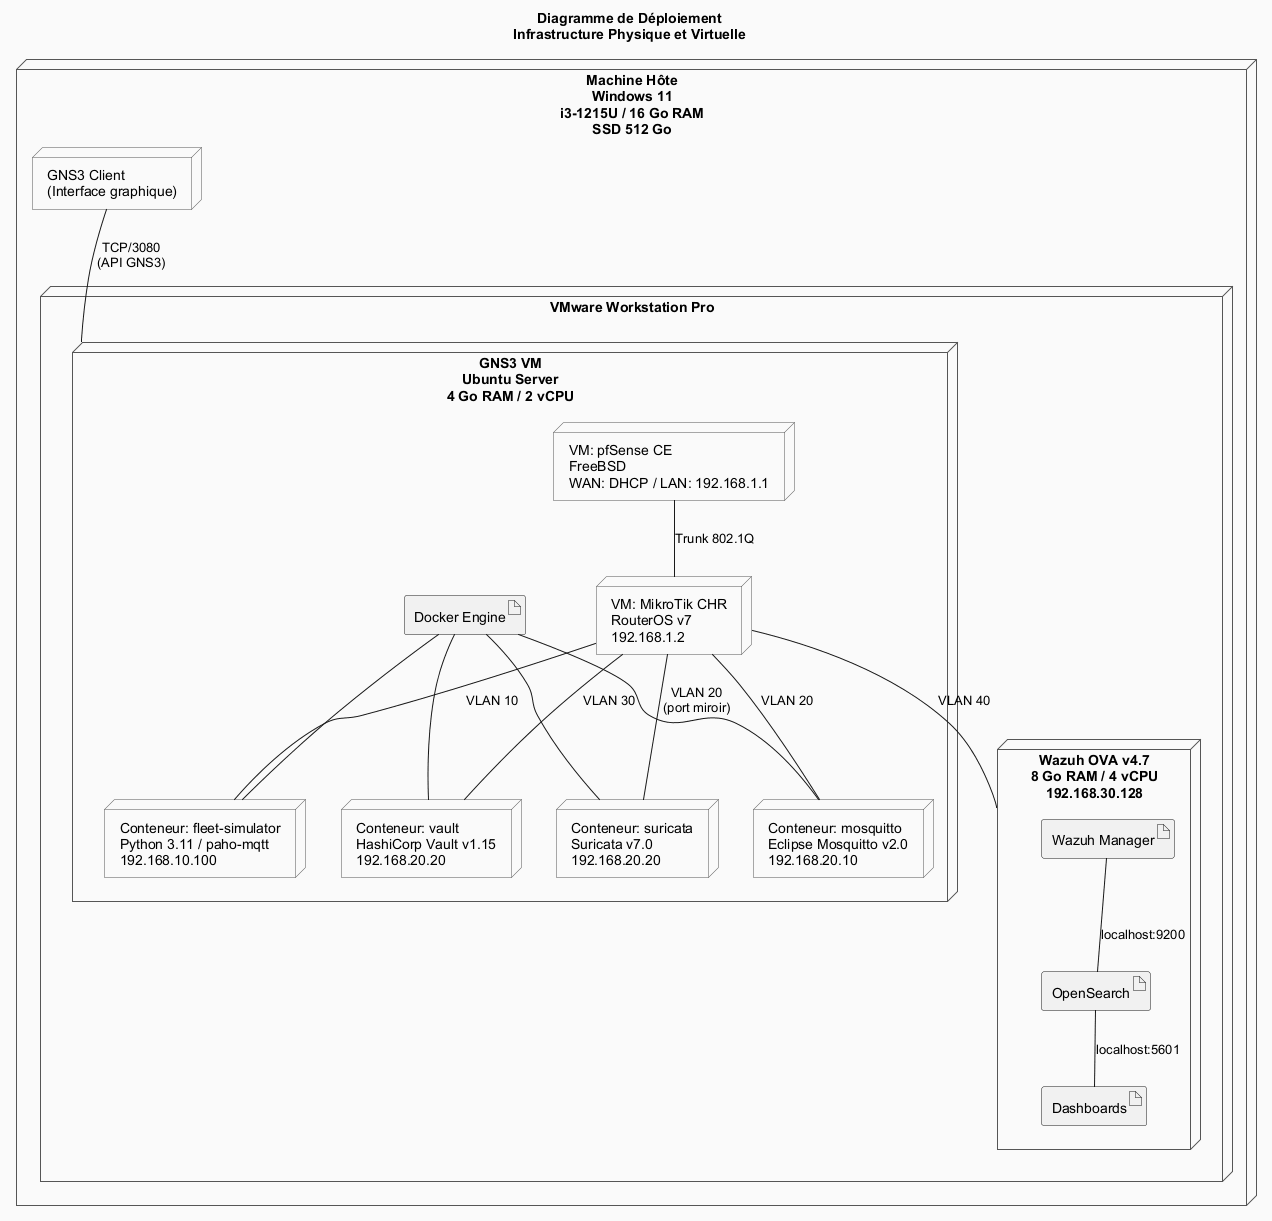
\includegraphics[width=\textwidth]{diagrams/diag-deploiement.png}
  \caption{Diagramme de déploiement -- infrastructure physique et virtuelle}
  \label{fig:deploiement}
\end{figure}

L'infrastructure s'appuie sur une machine hôte Windows~11 (Intel~i3-1215U, 16~Go de RAM) hébergeant VMware Workstation Pro. La VM GNS3 (Ubuntu Server, 4~Go de RAM) exécute le moteur Docker et les conteneurs applicatifs ; la VM Wazuh (OVA, 8~Go de RAM) est déployée séparément.

\section{Infrastructure PKI -- HashiCorp Vault}

\subsection{Hiérarchie de certification}

L'infrastructure PKI suit une hiérarchie à \textbf{deux niveaux} : une CA racine et une CA intermédiaire. Ce schéma est recommandé par le NIST (SP~800-57)~\cite{nist_sp800213} car il permet de garder la CA racine hors-ligne (réduction de la surface d'attaque), de remplacer la CA intermédiaire en cas de compromission sans invalider toute la chaîne, et de définir des politiques de certification distinctes par niveau. La figure~\ref{fig:pki_hierarchy} présente le diagramme de classes correspondant.

\begin{figure}[H]
  \centering
  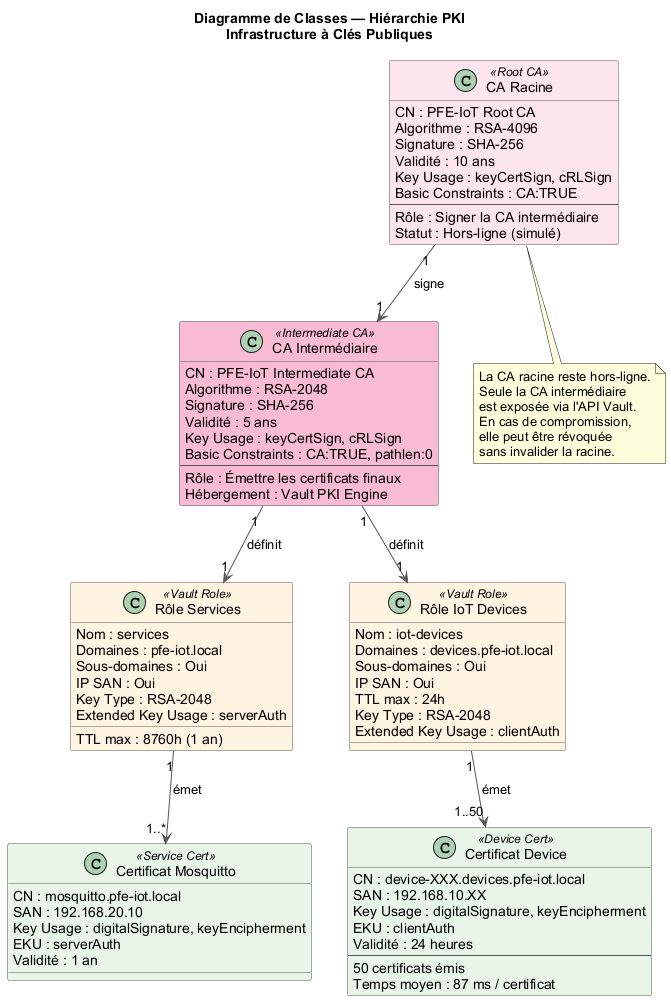
\includegraphics[width=0.8\textwidth]{diagrams/diag-pki-hierarchy.png}
  \caption{Hiérarchie PKI -- diagramme de classes}
  \label{fig:pki_hierarchy}
\end{figure}

\begin{table}[H]
\centering
\caption{Paramètres cryptographiques de la PKI}
\label{tab:pki_params}
\begin{tabular}{lll}
\toprule
\textbf{Paramètre} & \textbf{CA Racine} & \textbf{CA Intermédiaire} \\
\midrule
Algorithme de clé & RSA-4096 & RSA-2048 \\
Algorithme de signature & SHA-256 & SHA-256 \\
Durée de validité & 10~ans & 5~ans \\
Profil de certificat & CA basic constraint & CA basic constraint \\
\bottomrule
\end{tabular}
\end{table}

Pour les certificats \textbf{dispositifs et services} : RSA-2048/SHA-256, validité 24~heures pour les dispositifs IoT (renouvellement automatique), SAN incluant l'IP et le nom DNS, et Extended Key Usage \texttt{clientAuth} (dispositifs) ou \texttt{serverAuth} (Mosquitto).

\subsection{Déploiement de Vault et émission des certificats}

Vault~v1.15~\cite{vault_pki} est déployé dans un conteneur Docker basé sur l'image officielle \texttt{hashicorp/vault:1.15}. L'initialisation comprend la génération des clés de déverrouillage (\textit{unseal keys}) selon un schéma de Shamir (3~parts, seuil de 2), le déverrouillage avec deux clés, l'authentification avec le jeton racine, et l'activation du moteur PKI racine. La CA racine est générée en interne (Common~Name : \texttt{PFE-IoT Root~CA}, RSA-4096, validité 10~ans). La CA intermédiaire est créée en trois étapes : génération du CSR par le moteur \texttt{pki\_int}, signature par la CA racine, puis import du certificat signé.

Deux rôles d'émission sont définis pour contrôler les types de certificats :

\begin{table}[H]
\centering
\caption{Rôles d'émission PKI définis dans Vault}
\label{tab:vault_roles}
\begin{tabular}{llll}
\toprule
\textbf{Rôle} & \textbf{Domaine autorisé} & \textbf{TTL max} & \textbf{Usage} \\
\midrule
\texttt{services} & \texttt{pfe-iot.local} & 1~an & Mosquitto, Vault \\
\texttt{iot-devices} & \texttt{devices.pfe-iot.local} & 24~h & Dispositifs IoT \\
\bottomrule
\end{tabular}
\end{table}

Le processus d'émission automatique d'un certificat de dispositif est illustré par le diagramme de séquence de la figure~\ref{fig:pki_sequence}. Pour chaque dispositif simulé, le script \texttt{generate\_device\_certs.sh} (Annexe~A, section~\ref{sec:script_gen_certs}) effectue un appel API REST au endpoint \texttt{/v1/pki\_int/issue/iot-devices}. La réponse contient le certificat X.509, la clé privée et la chaîne de certification (CA intermédiaire + racine).

\begin{figure}[H]
  \centering
  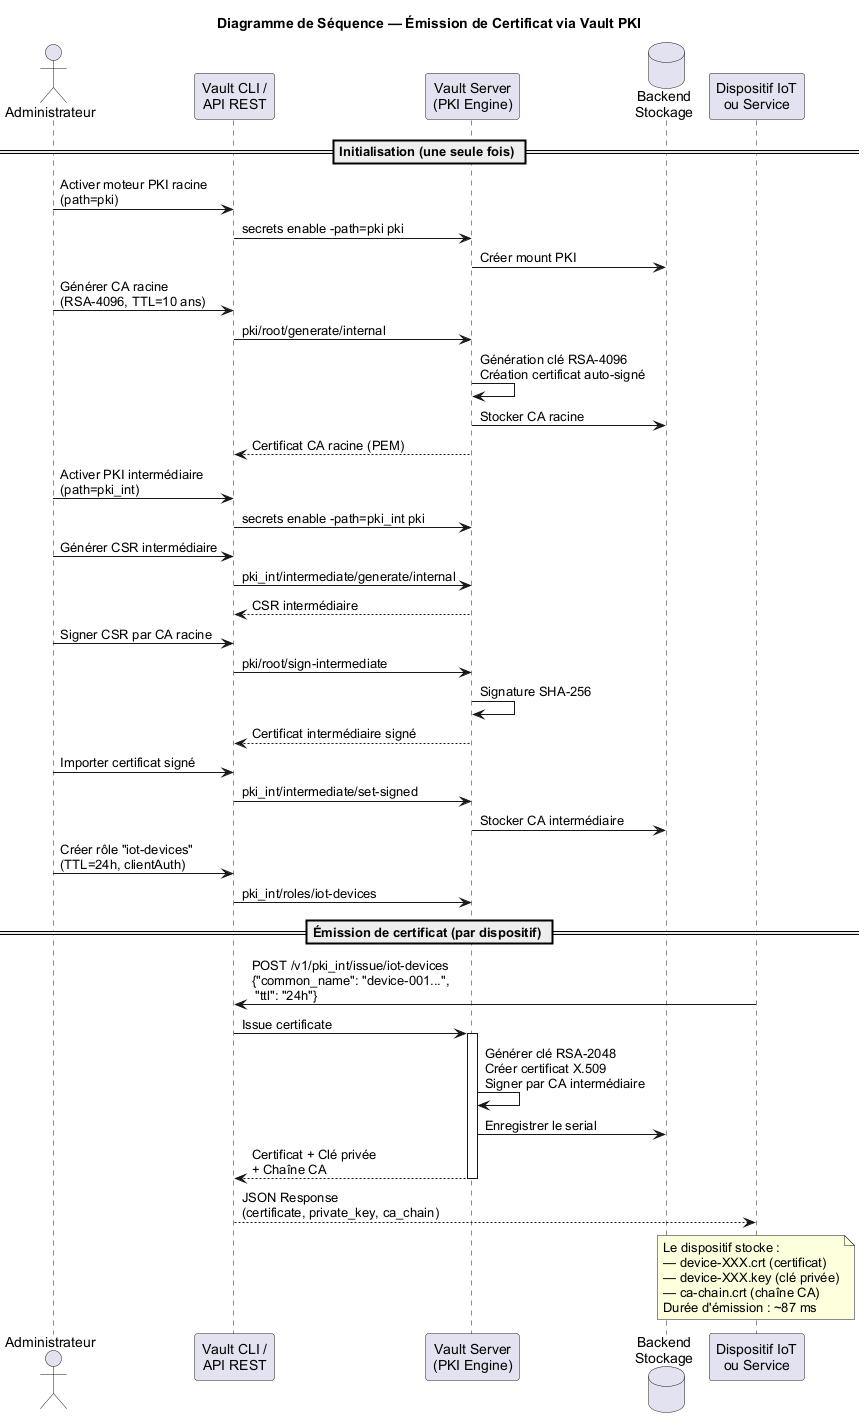
\includegraphics[width=0.85\textwidth]{diagrams/diag-pki-sequence.png}
  \caption{Séquence d'émission d'un certificat via l'API Vault}
  \label{fig:pki_sequence}
\end{figure}

\begin{resultbox}[Résultat PKI]
\textbf{50 certificats de dispositifs} émis avec succès via l'API Vault. Chaîne de confiance validée : dispositif $\to$ CA intermédiaire $\to$ CA racine. Durée d'émission moyenne : \textbf{87~ms} par certificat via API REST.
\end{resultbox}

\section{Configuration TLS/mTLS sur Mosquitto}

\subsection{Architecture de sécurité}

Eclipse Mosquitto~v2.0~\cite{mosquitto_tls} est déployé en conteneur Docker sur la zone Services (192.168.20.10). Quatre principes fondamentaux structurent sa configuration : désactivation complète du port non chiffré (1883) au profit du seul port 8883, TLS~1.3 obligatoire (versions antérieures interdites), mTLS obligatoire (\texttt{require\_certificate true}), et ACL liée au \textbf{Common~Name} du certificat client.

\begin{table}[H]
\centering
\caption{Directives principales de sécurité Mosquitto}
\label{tab:mosquitto_directives}
\begin{tabular}{llp{5.5cm}}
\toprule
\textbf{Directive} & \textbf{Valeur} & \textbf{Description} \\
\midrule
\texttt{listener} & 8883 & Port unique TLS \\
\texttt{cafile} & \texttt{ca-chain.crt} & Chaîne CA de confiance \\
\texttt{certfile} & \texttt{server.crt} & Certificat du serveur \\
\texttt{keyfile} & \texttt{server.key} & Clé privée du serveur \\
\texttt{require\_certificate} & \texttt{true} & mTLS obligatoire \\
\texttt{use\_identity\_as\_username} & \texttt{true} & CN comme identifiant MQTT \\
\texttt{tls\_version} & \texttt{tlsv1.3} & TLS~1.3 strict \\
\texttt{allow\_anonymous} & \texttt{false} & Connexions anonymes interdites \\
\bottomrule
\end{tabular}
\end{table}

Le fichier ACL associe le CN du certificat client aux topics autorisés : chaque dispositif IoT dispose d'un espace de noms dédié (\texttt{iot/sensors/<device-id>/\#} en publication, \texttt{iot/commands/<device-id>/\#} en souscription). La configuration complète est fournie en Annexe~B (section~\ref{sec:config_mosquitto}).

\subsection{Validation et analyse du handshake}

La validation s'effectue en deux temps. Le \textbf{test négatif} consiste à tenter une connexion sans certificat client : le broker rejette avec une erreur \texttt{SSL alert handshake failure}, confirmant l'effectivité du mTLS. Le \textbf{test positif} avec un certificat valide aboutit à une session TLS~1.3 négociée avec la cipher suite \texttt{TLS\_AES\_256\_GCM\_SHA384}. Un test fonctionnel \textit{publish/subscribe} via \texttt{mosquitto\_pub} et \texttt{mosquitto\_sub} valide ensuite le routage par topic et la réception du message.

La figure~\ref{fig:tls_handshake} détaille les échanges du handshake TLS~1.3 mTLS, capturé via Wireshark. Le tableau~\ref{tab:handshake_tls} présente la décomposition temporelle de chaque étape.

\begin{figure}[H]
  \centering
  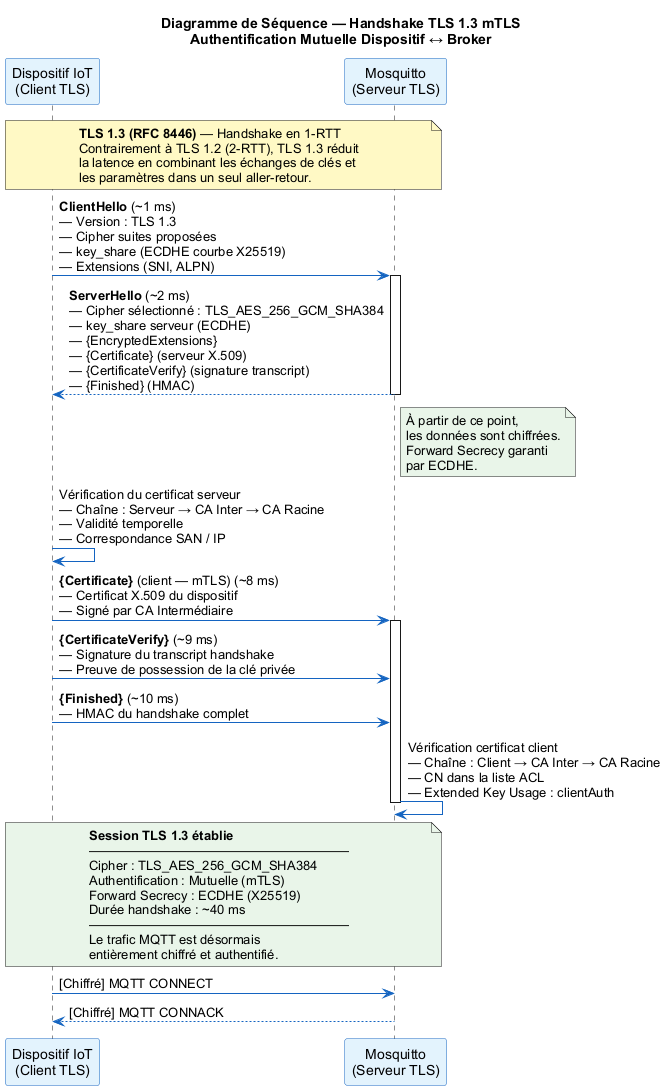
\includegraphics[width=0.7\textwidth]{diagrams/diag-tls-handshake.png}
  \caption{Handshake TLS~1.3 mTLS -- diagramme de séquence détaillé}
  \label{fig:tls_handshake}
\end{figure}

\begin{table}[H]
\centering
\caption{Analyse temporelle du handshake TLS~1.3 en mTLS}
\label{tab:handshake_tls}
\begin{tabular}{llp{6cm}}
\toprule
\textbf{Étape} & \textbf{Durée} & \textbf{Description} \\
\midrule
ClientHello & $<$ 1~ms & Propose TLS~1.3, cipher suites, \texttt{key\_share} \\
ServerHello & $\sim$2~ms & Sélection \texttt{TLS\_AES\_256\_GCM\_SHA384} \\
EncryptedExtensions & $\sim$3~ms & Extensions chiffrées (ALPN, SNI) \\
Certificate (serveur) & $\sim$5~ms & Certificat X.509 du broker \\
CertificateVerify & $\sim$6~ms & Signature du transcript par le serveur \\
Finished (serveur) & $\sim$7~ms & HMAC du handshake \\
Certificate (client) & $\sim$8~ms & Certificat X.509 du dispositif (mTLS) \\
CertificateVerify & $\sim$9~ms & Signature par le dispositif \\
Finished (client) & $\sim$10~ms & Établissement complet de la session \\
\bottomrule
\end{tabular}
\end{table}

\begin{resultbox}[Résultat TLS/mTLS]
Durée totale du handshake TLS~1.3 mTLS : \textbf{$\sim$40~ms}.\\
Cipher suite sélectionnée : \texttt{TLS\_AES\_256\_GCM\_SHA384}.\\
Toutes les connexions sans certificat client valide sont rejetées.\\
50 dispositifs connectés simultanément sans dégradation notable.
\end{resultbox}

\section{Conclusion}

Ce chapitre a détaillé la réalisation des trois piliers de l'infrastructure : la topologie réseau segmentée sous GNS3, la PKI dynamique HashiCorp Vault à deux niveaux, et la configuration durcie du broker Mosquitto en TLS~1.3/mTLS. Les 50 certificats émis, le handshake mTLS de 40~ms et le rejet systématique des connexions non authentifiées valident le bon fonctionnement de la chaîne cryptographique. Le chapitre suivant exploite cette base pour simuler le trafic d'une flotte IoT réaliste et l'analyser via Suricata et Wazuh.
